\documentclass[12pt]{beamer}
\usepackage{xspace}
\usepackage{listings}
\lstset{
  basicstyle=\footnotesize,
  numbers=left,
  numberstyle=\tiny,
%  frame=single,
  columns=flexible
}
\usepackage{graphicx}
\newcommand{\mint}{{\sffamily\scshape mint}\xspace}

\title{The \mint neural network library}
\author[S Ghirlanda]{Stefano Ghirlanda}
\subtitle{A quick introduction}
\date{June 7\textsuperscript{th}, 2011}

\begin{document}

\begin{frame}
  \titlepage
\end{frame}

\begin{frame}{Why neural networks}
  \begin{center}
    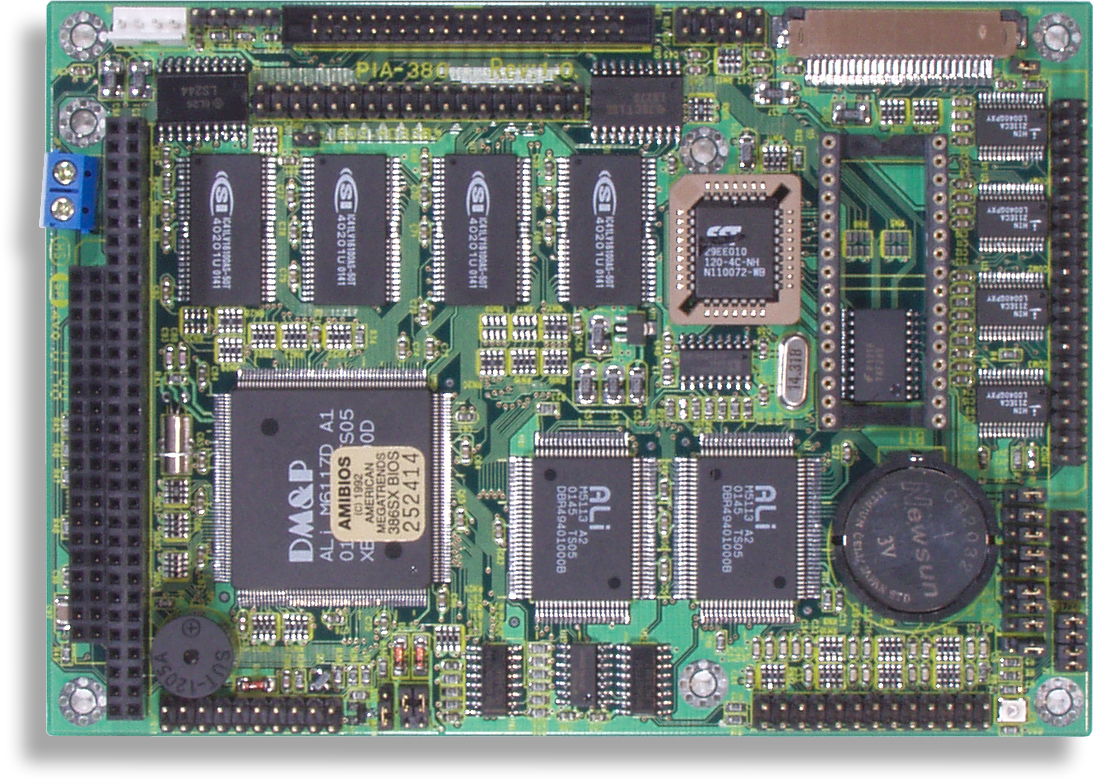
\includegraphics[width=.35\textwidth]{circuitBoard}\hspace{3ex}
    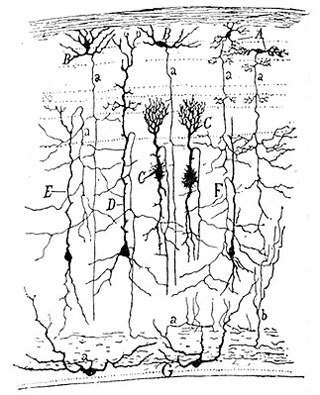
\includegraphics[width=.25\textwidth]{sparrowOpticTectum}
  \end{center}

  \begin{itemize}
  \item Dominant paradigm for understanding intelligence:\\ the
    digital computer
  \item Natural intelligence is done by brains
  \item Neural networks try to capture the ``computational style''
    of brains
  \end{itemize}

  \vfill

\end{frame}

\begin{frame}{Neural networks in a nutshell}
  \begin{itemize}
  \item<1-> Made of ``nodes'' (neurons) that can be in different
    states of activity (on-off, between 0 and 1, etc.)
  \item<1-> Nodes influence each other through ``connection weights''
    (synapses) which can be positive/negative (excitatory/inhibitory),
    strong or weak
  \item<1-> Some nodes are ``input'' (sensors), others ``ouptut'' (e.g., motor neurons)
  \item<2-> Node activity changes in time reflecting input values and characteristics of the network 
  \item<2-> Connections may change, too (``learning'')
  \item<3-> \textbf{Goal: understanding how all this generates
      behavior!}
  \end{itemize}
  
\end{frame}

\begin{frame}{Why \mint}
  \begin{itemize}
  \item Computer simulation is crucial in neural network modeling
  \item Problems of existing software:
    \begin{itemize}
    \item Engineering view of neural networks
    \item Not general
    \item Too low level for my (our) purpose
    \item Makes things complicated
    \item Costs money
    \end{itemize}
  \end{itemize}
\end{frame}

\begin{frame}{Example}
  \begin{center}
  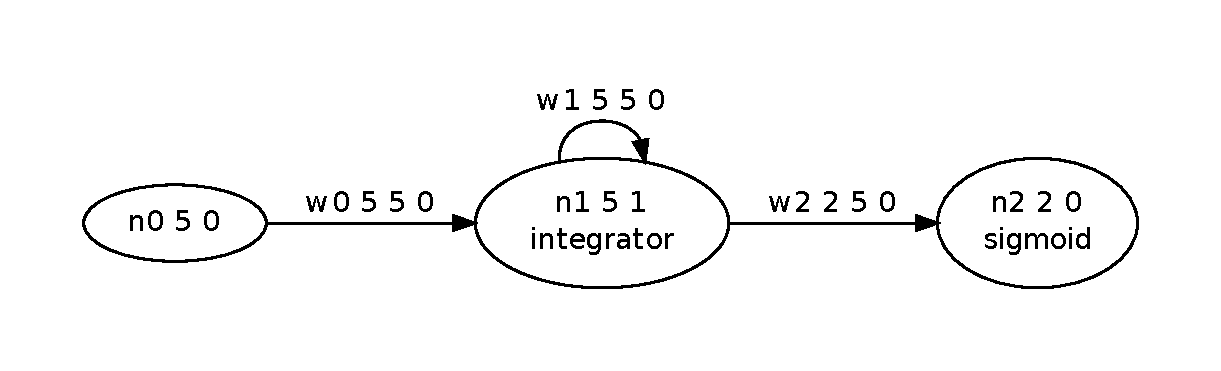
\includegraphics[width=\textwidth]{recnetGraph}
  \pause
  \lstinputlisting{recnet/recnet.arc}    
  \end{center}
  \vfill
\end{frame}

\begin{frame}{``Integrator'' and ``sigmoid''}
  \begin{center}
    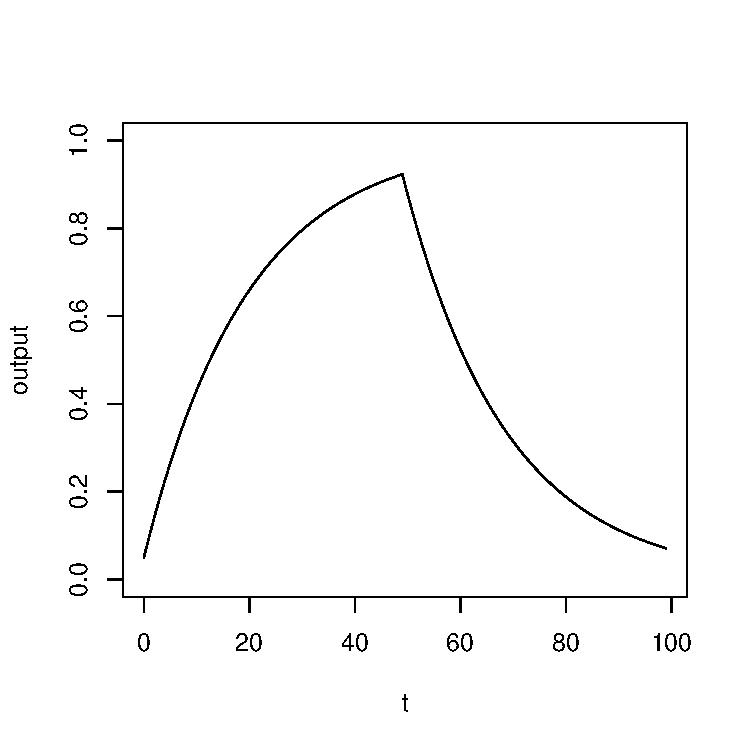
\includegraphics[width=.45\textwidth]{integrator}    
    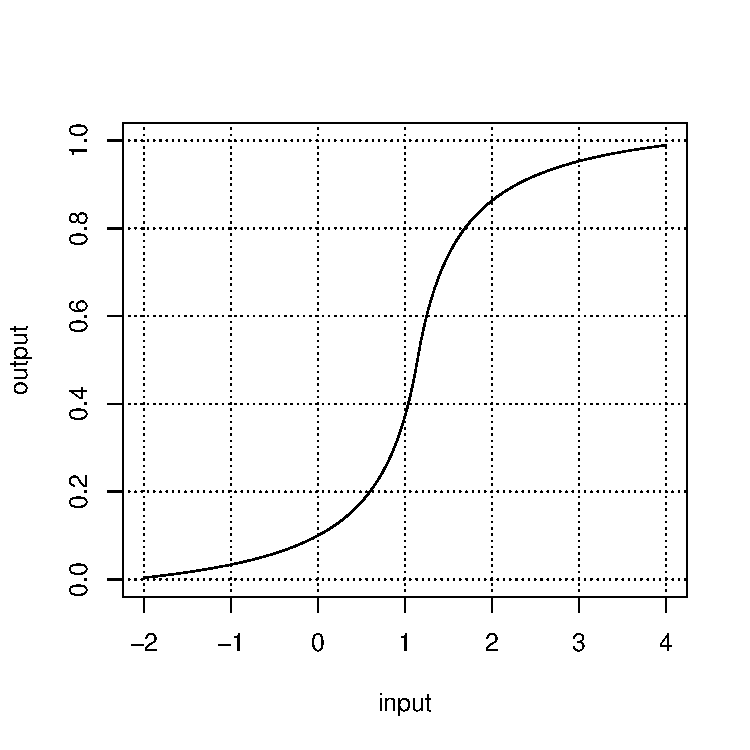
\includegraphics[width=.45\textwidth]{sigmoid}    
  \end{center}
\end{frame}

\begin{frame}[fragile]{Code}
  Creating the network:
  \lstinputlisting[columns=fullflexible,linerange={18-18,24-26}]{%
    recnet/recnet.c}
  \pause
  Setting the weights:
  \lstinputlisting[columns=fullflexible,linerange={28-30}]{recnet/recnet.c}
  \pause
  Running the network:
  \lstinputlisting[columns=fullflexible,linerange={44-47,53-53}]{%
    recnet/recnet.c}
\end{frame}

\begin{frame}{Results}
  ``Brain'' activity in response to constant input:
  \begin{center}
    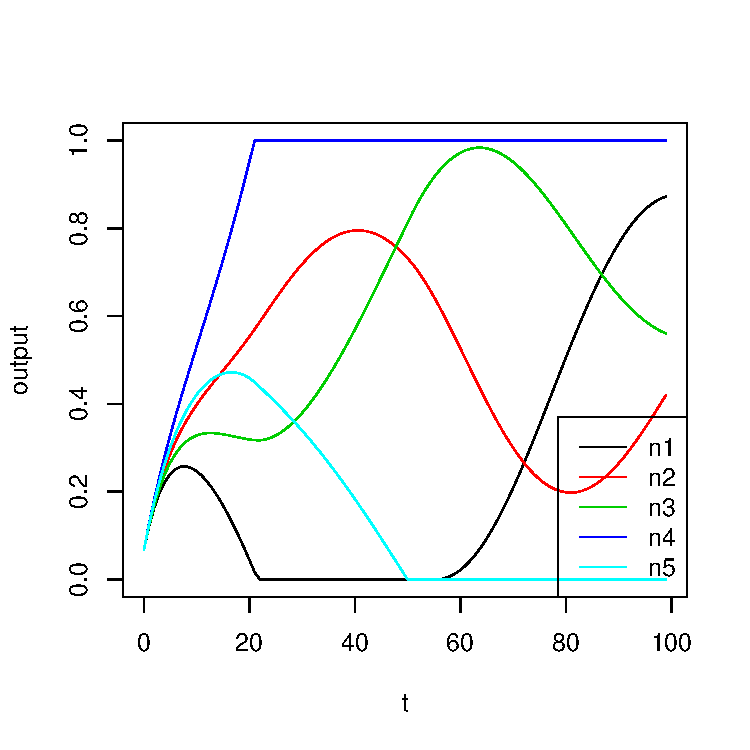
\includegraphics[width=.7\textwidth]{recnetGood2}
  \end{center}
  \vfill
\end{frame}

\begin{frame}[fragile]{Analysis}
  \ldots
  \lstinputlisting[columns=flexible,linerange={25-30}]{recnet/recnetDetailGood2.arc}
  \ldots
\end{frame}

\begin{frame}{What next}
  \begin{itemize}
  \item Documentation
  \item Testing
  \item Features:
    \begin{itemize}
    \item Learning
    \item Analysis / Visualization
    \item Interfacing with Khepera
    \item \ldots
    \end{itemize}

  \end{itemize}
\end{frame}
\end{document}
